% anhang.tex
\chapter{Weitere Informationen}
\section{Alternative Eingabedaten}
\begin{figure}
    \centering
    \caption{Laufzeitmessung von LZ77, Approx.LZ77 und Approx.LZ77Par(16 Threads) auf verschiedenen Präfixen von sources. Als Vergleichsmaß wurde 
    die lineare Regression der Kurven gestrichelt eingezeichnet.}
    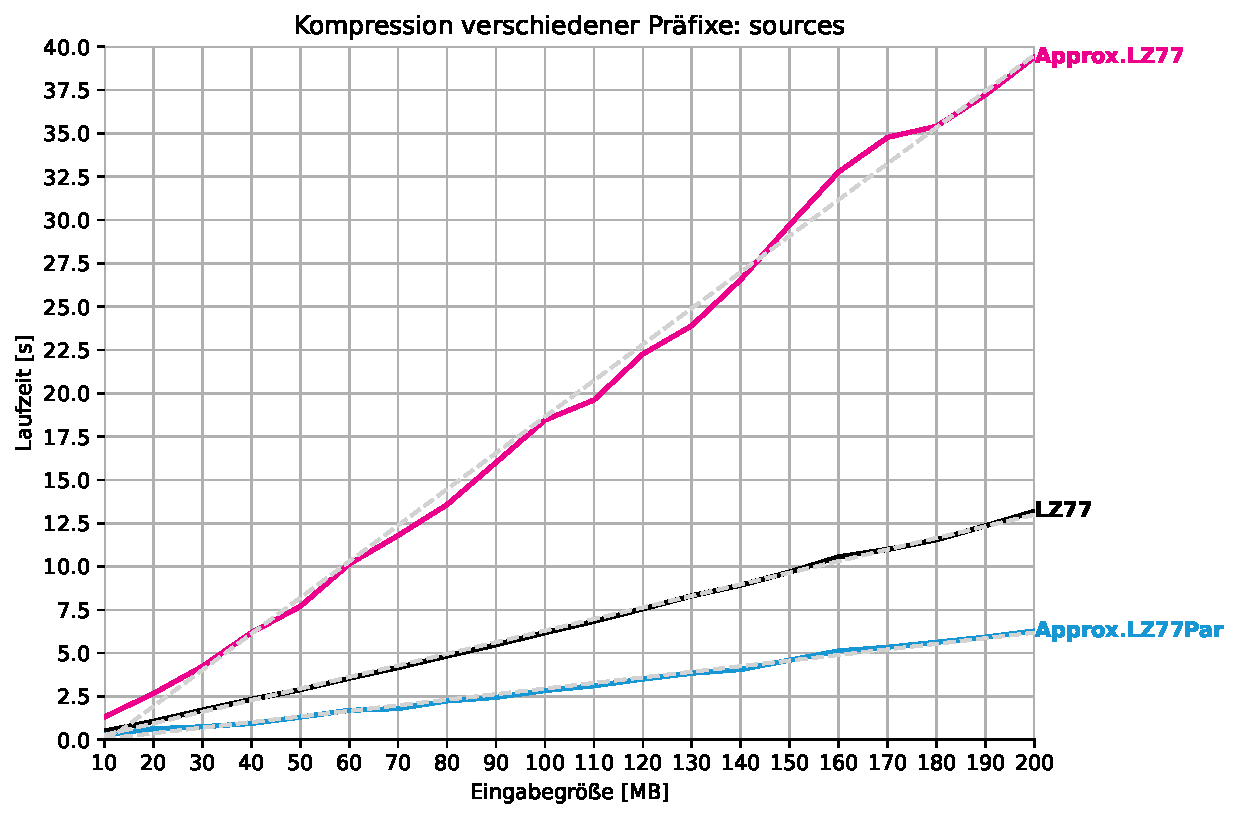
\includegraphics[scale=0.6]{Images/progressive_sources.pdf}
\end{figure}

\begin{figure}
    \centering
    \caption{Laufzeitmessung von Approx.LZ77Par mit verschiedener Anzahl an Threads für sources}
    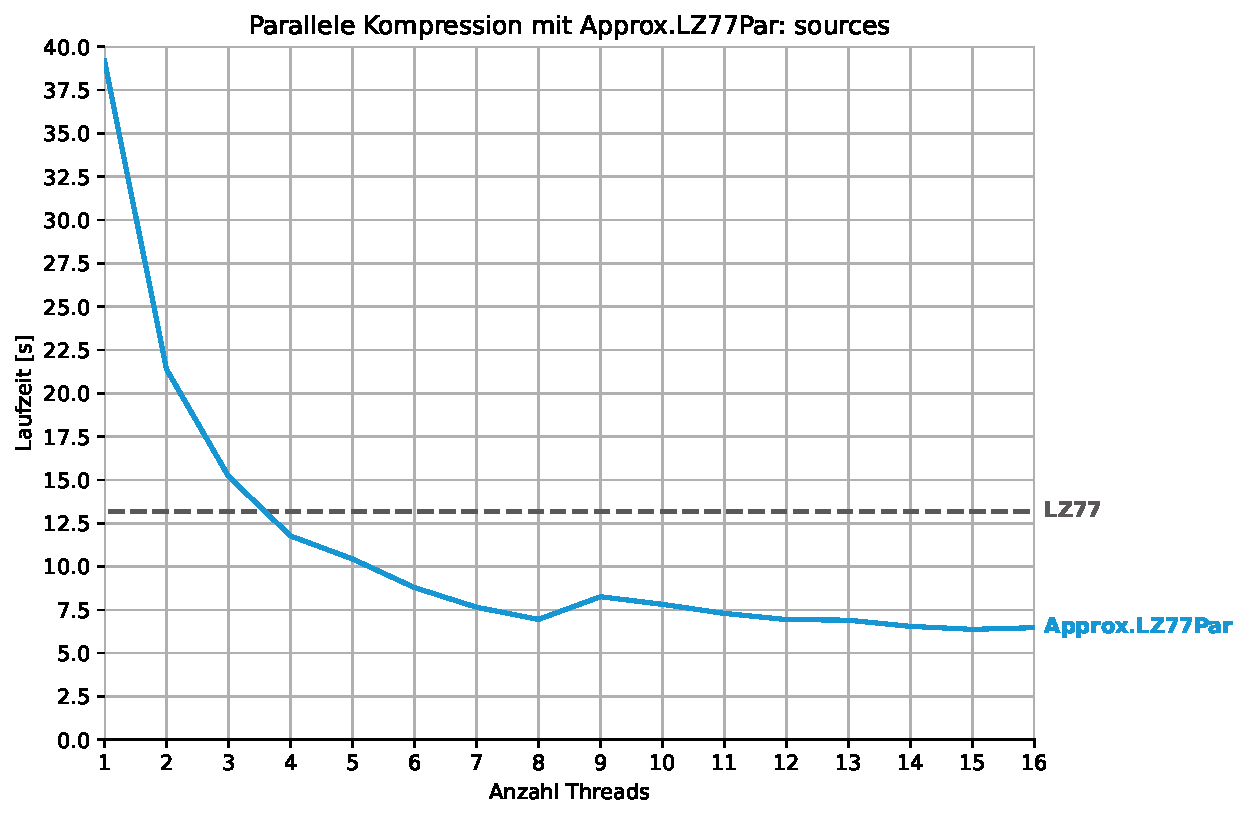
\includegraphics[scale=0.6]{Images/progressive_speedup_sources.pdf}
\end{figure}

\begin{figure}
    \centering
    \caption{Laufzeitmessung von LZ77, Approx.LZ77 und Approx.LZ77Par(16 Threads) auf verschiedenen Präfixen von english. Als Vergleichsmaß wurde 
    die lineare Regression der Kurven gestrichelt eingezeichnet.}
    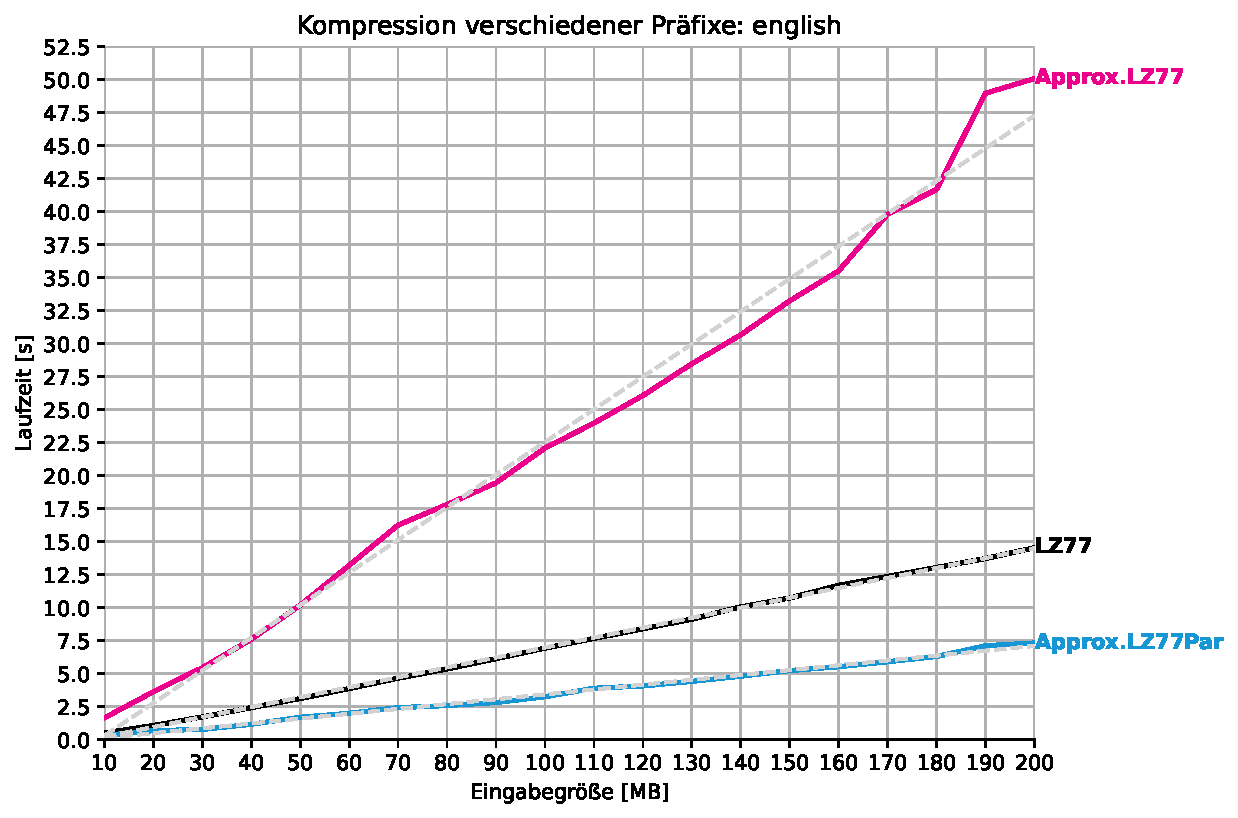
\includegraphics[scale=0.6]{Images/progressive_english.pdf}
\end{figure}

\begin{figure}
    \centering
    \caption{Laufzeitmessung von Approx.LZ77Par mit verschiedener Anzahl an Threads für english}
    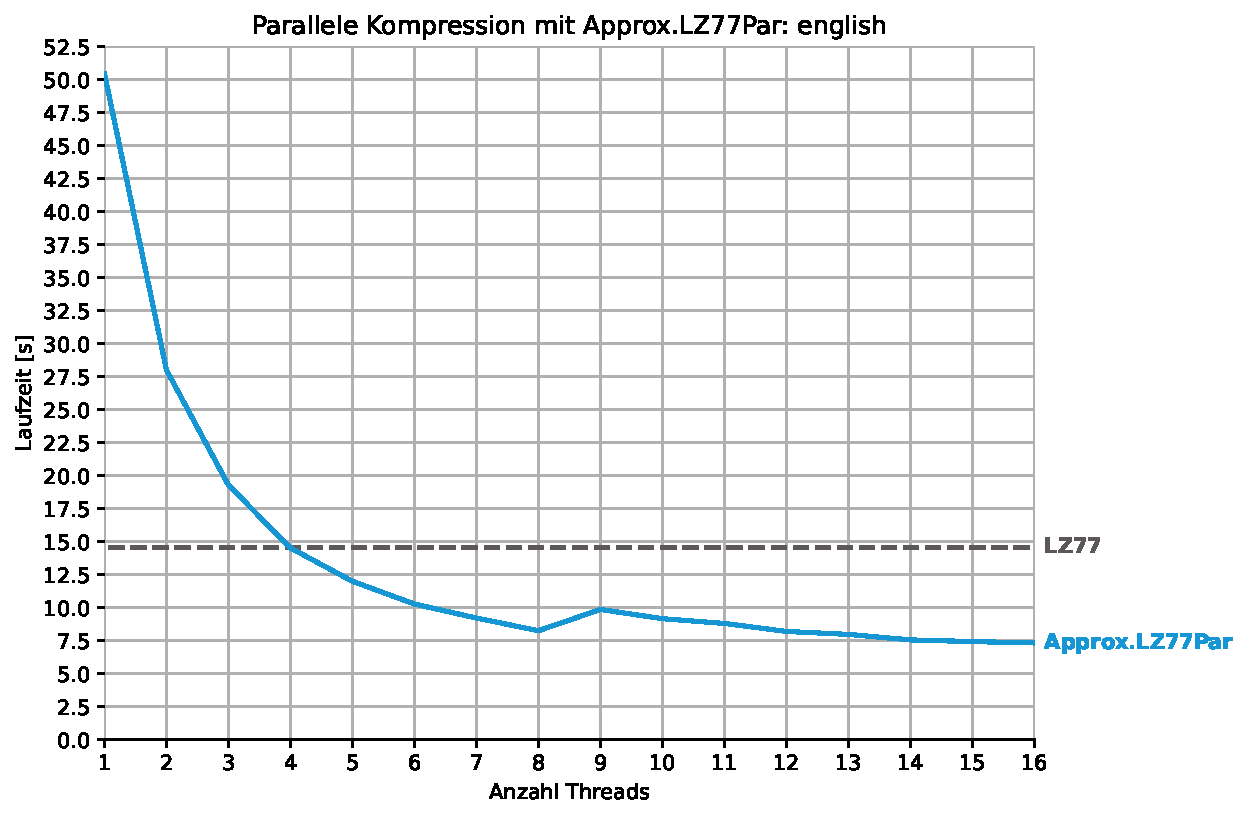
\includegraphics[scale=0.6]{Images/progressive_speedup_english.pdf}
\end{figure}

\begin{figure}
    \centering
    \caption{Laufzeitmessung von LZ77, Approx.LZ77 und Approx.LZ77Par(16 Threads) auf verschiedenen Präfixen von dna. Als Vergleichsmaß wurde 
    die lineare Regression der Kurven gestrichelt eingezeichnet.}
    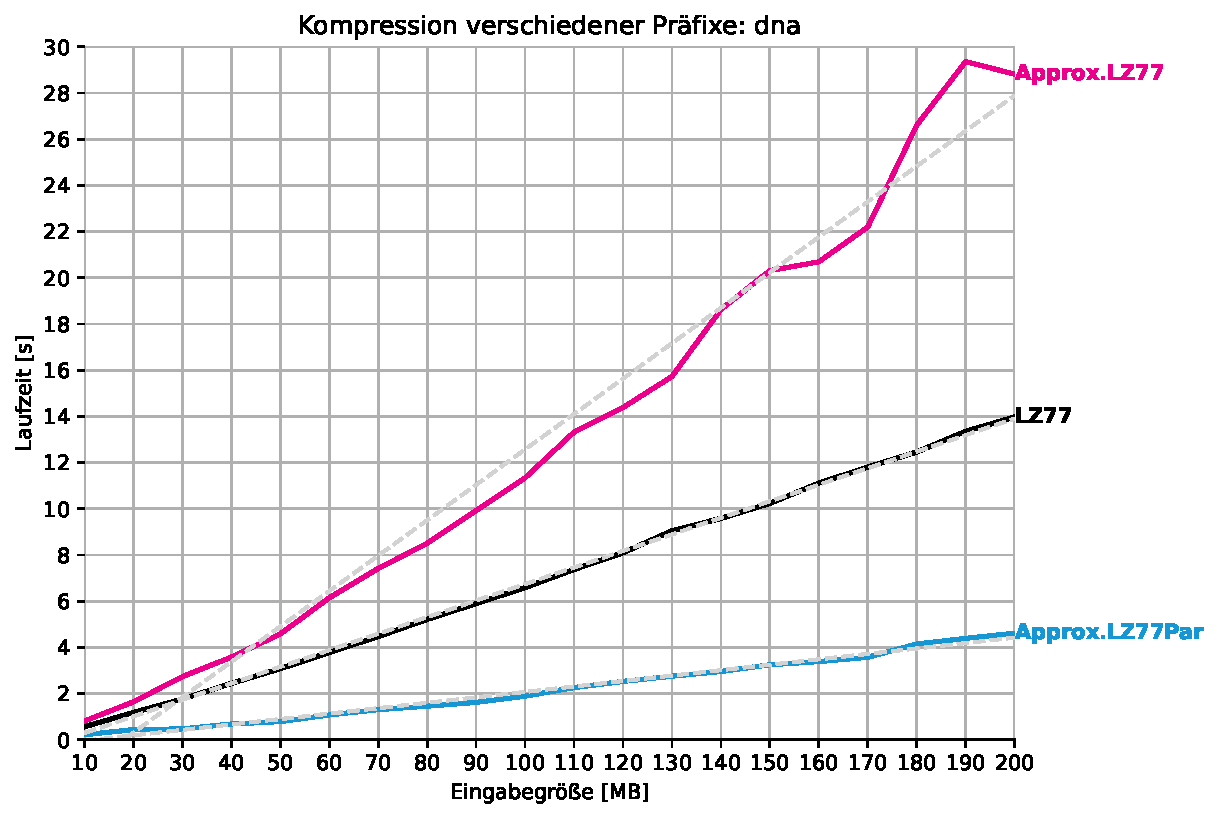
\includegraphics[scale=0.6]{Images/progressive_dna.pdf}
\end{figure}

\begin{figure}
    \centering
    \caption{Laufzeitmessung von Approx.LZ77Par mit verschiedener Anzahl an Threads für dna}
    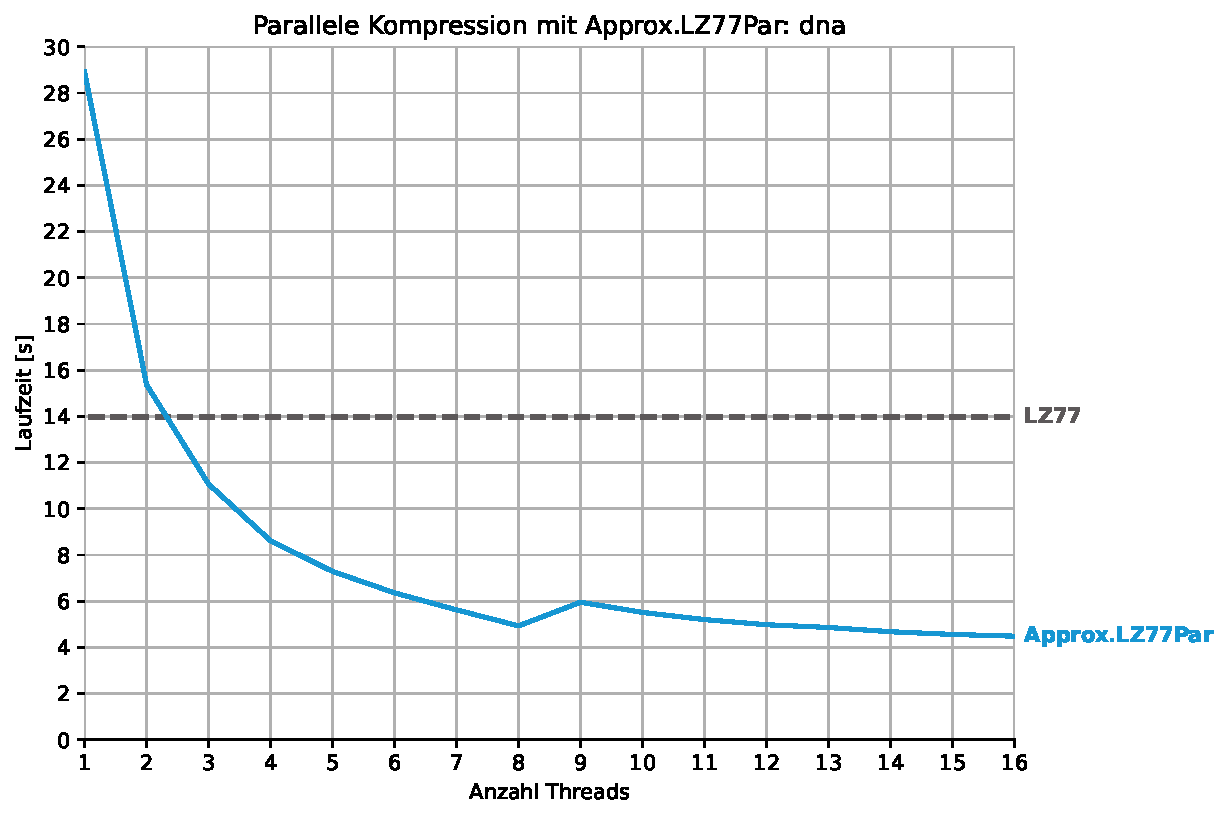
\includegraphics[scale=0.6]{Images/progressive_speedup_dna.pdf}
\end{figure}

\begin{figure}
    \centering
    \caption{Laufzeitmessung von LZ77, Approx.LZ77 und Approx.LZ77Par(16 Threads) auf verschiedenen Präfixen von xml. Als Vergleichsmaß wurde 
    die lineare Regression der Kurven gestrichelt eingezeichnet.}
    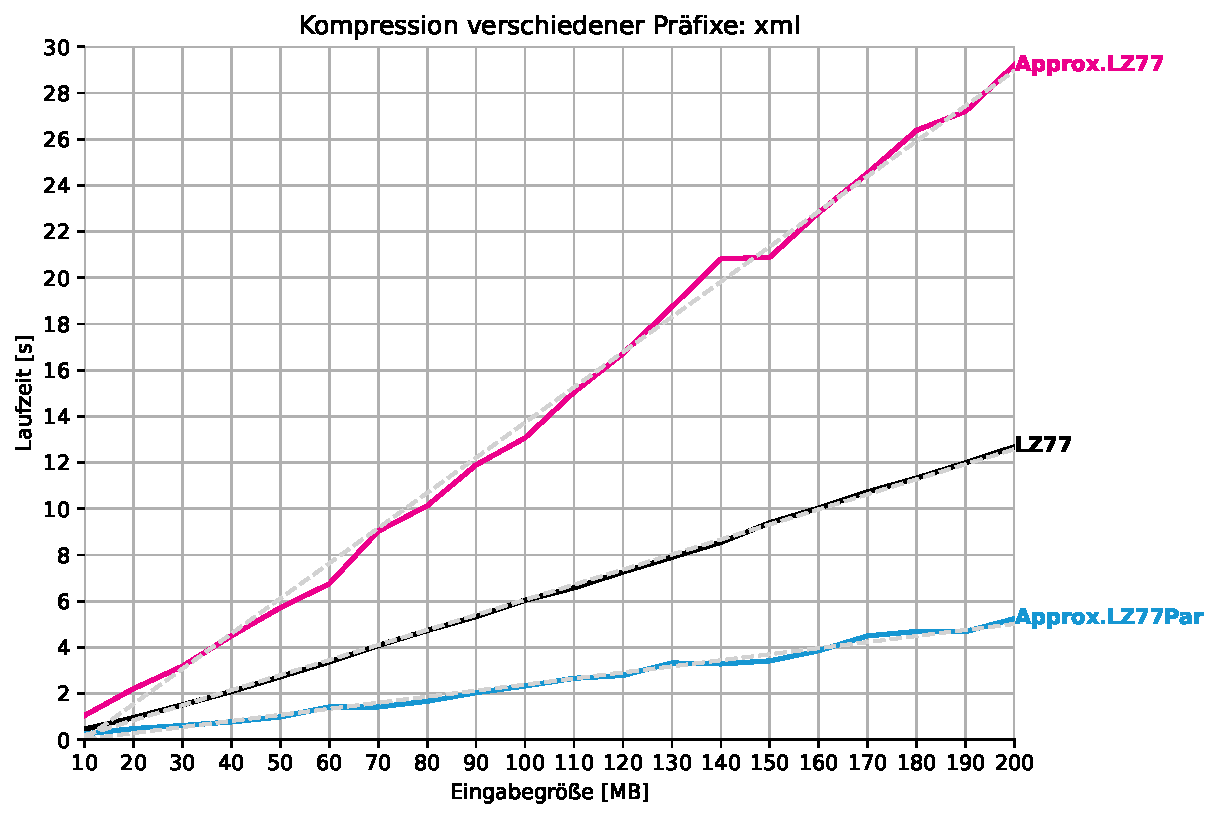
\includegraphics[scale=0.6]{Images/progressive_xml.pdf}
\end{figure}

\begin{figure}
    \centering
    \caption{Laufzeitmessung von Approx.LZ77Par mit verschiedener Anzahl an Threads für xml}
    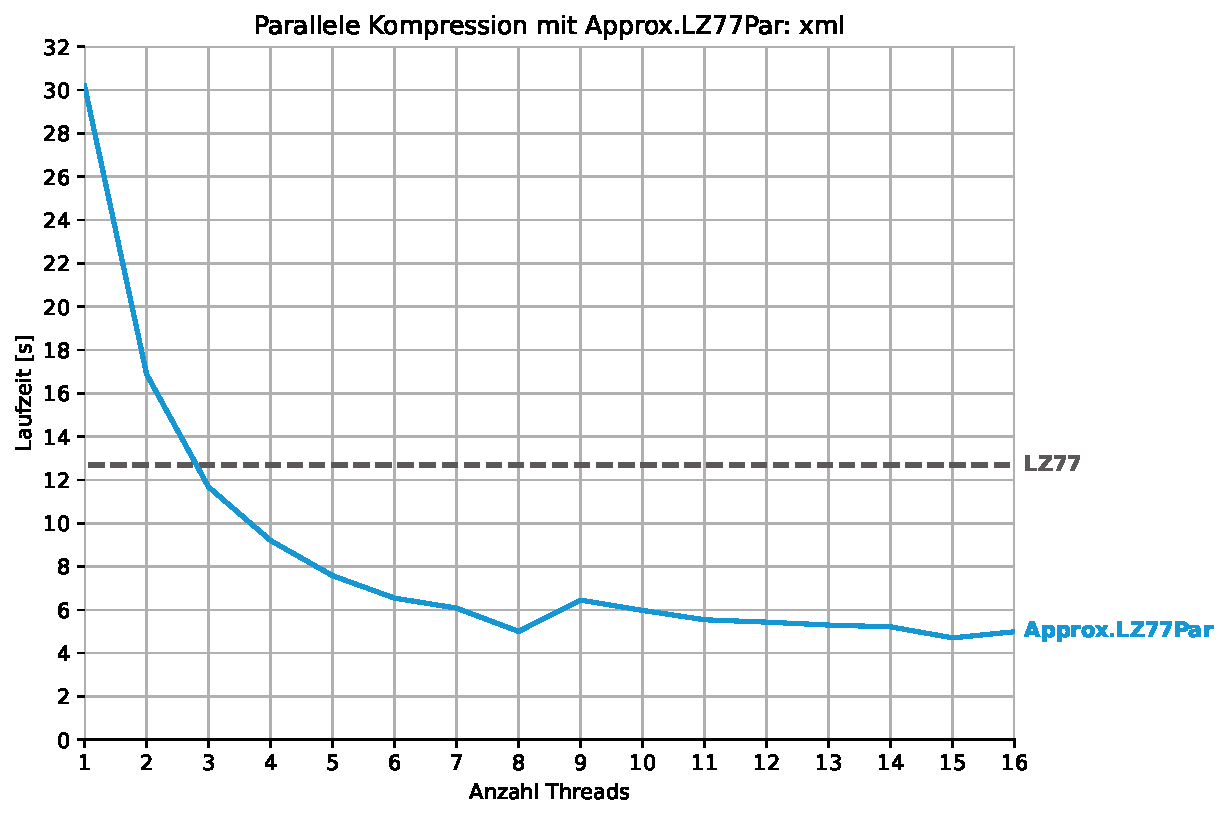
\includegraphics[scale=0.6]{Images/progressive_speedup_xml.pdf}
\end{figure}

\section{Alternative Testumgebung}